\newpage
\section{Replication: Synchronizing State}

This section discusses replicating state across distributed systems.

\begin{Def}[Replication]

    \textbf{Replication} is the process of maintaining multiple copies of the same data on different nodes (machines). 
    This is done for fault-tolerance, load balancing, and data locality.
\end{Def}

\noindent
\textbf{Problem Space:}\\
Consider we are running a money transfer service, from which Alice and Bob interact with:
\begin{figure}[h]
    \centering
    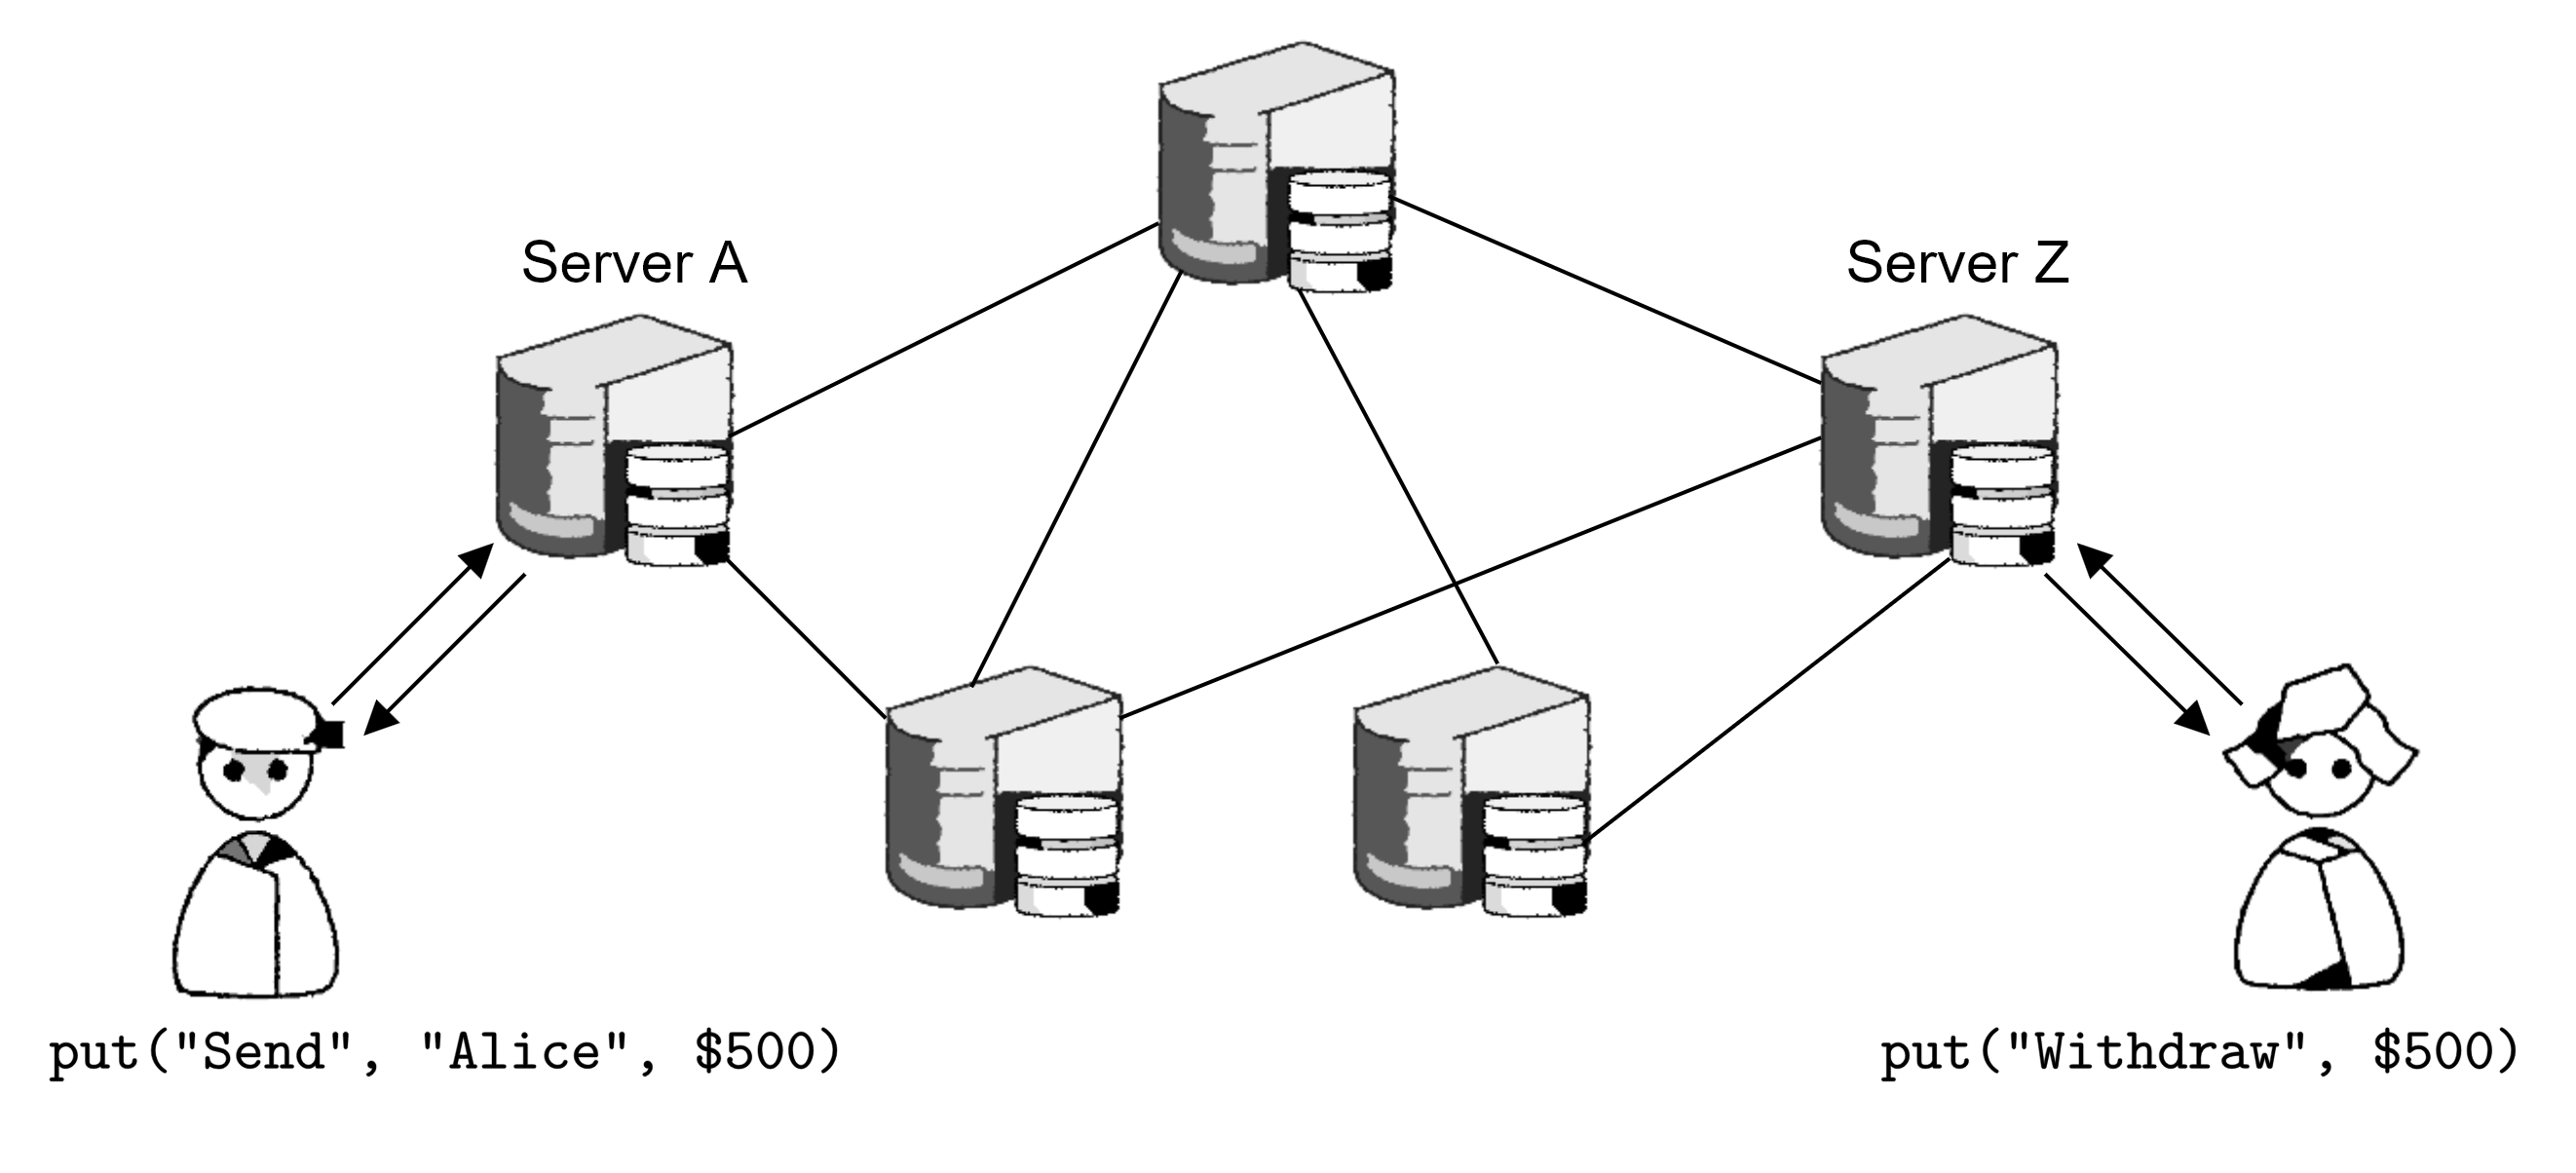
\includegraphics[width=.9\textwidth]{Sections/rep/intro.png}
    \caption{Bob sending money to Alice, while she withdraws money on two different servers.}
\end{figure}

\noindent
In this scenario Many problems can arise: What if,
\begin{itemize}
    \item The respective servers crash while or after Alice or Bob make requests?
    \item Alice and Bob share the same account, how do we ensure consistency?
\end{itemize}

\noindent
In all, wow do we ensure the propagation and synchronization of state across multiple servers?
We consider two models:
\begin{Def}[Active vs. Passive Replication]

    \textbf{Active Replication}: Client sends requests to all servers at the same time and waits for acknowledgments. This method must ensure that all 
    requests are processed in the same order (expensive).\\
    
    \noindent
    \textbf{Passive Replication}: Client sends requests to a primary server, which then forwards the request to backup servers.
\end{Def}

\newpage 

\noindent
We'll be move forward with \textbf{Passive Replication} as the preferred choice in this section.
Though it is less expensive than active replication, it still has its challenges:
\begin{itemize}
    \item \textbf{Consistency}: How do we ensure all backups are consistent?
    \item \textbf{Failure Handling}: What if the primary server fails?
    \item \textbf{Performance}: How do we ensure that the system is performant as we scale backups?
\end{itemize}

\noindent
We consider two methods of replication:
\begin{Def}[State vs. Request Replication]

    \textbf{State Replication}: Forward the entire state to backups. This results in large message sizes, but is relatively simple depending on the system.\\

    \noindent 
    \textbf{Request Replication}: Forward only requests to backups. This results in smaller message sizes, but adds complexity when requests are not deterministic (e.g., random number generation).
\end{Def}

\noindent
Still again, we run into the following problem:
\begin{figure}[h]
    \centering
    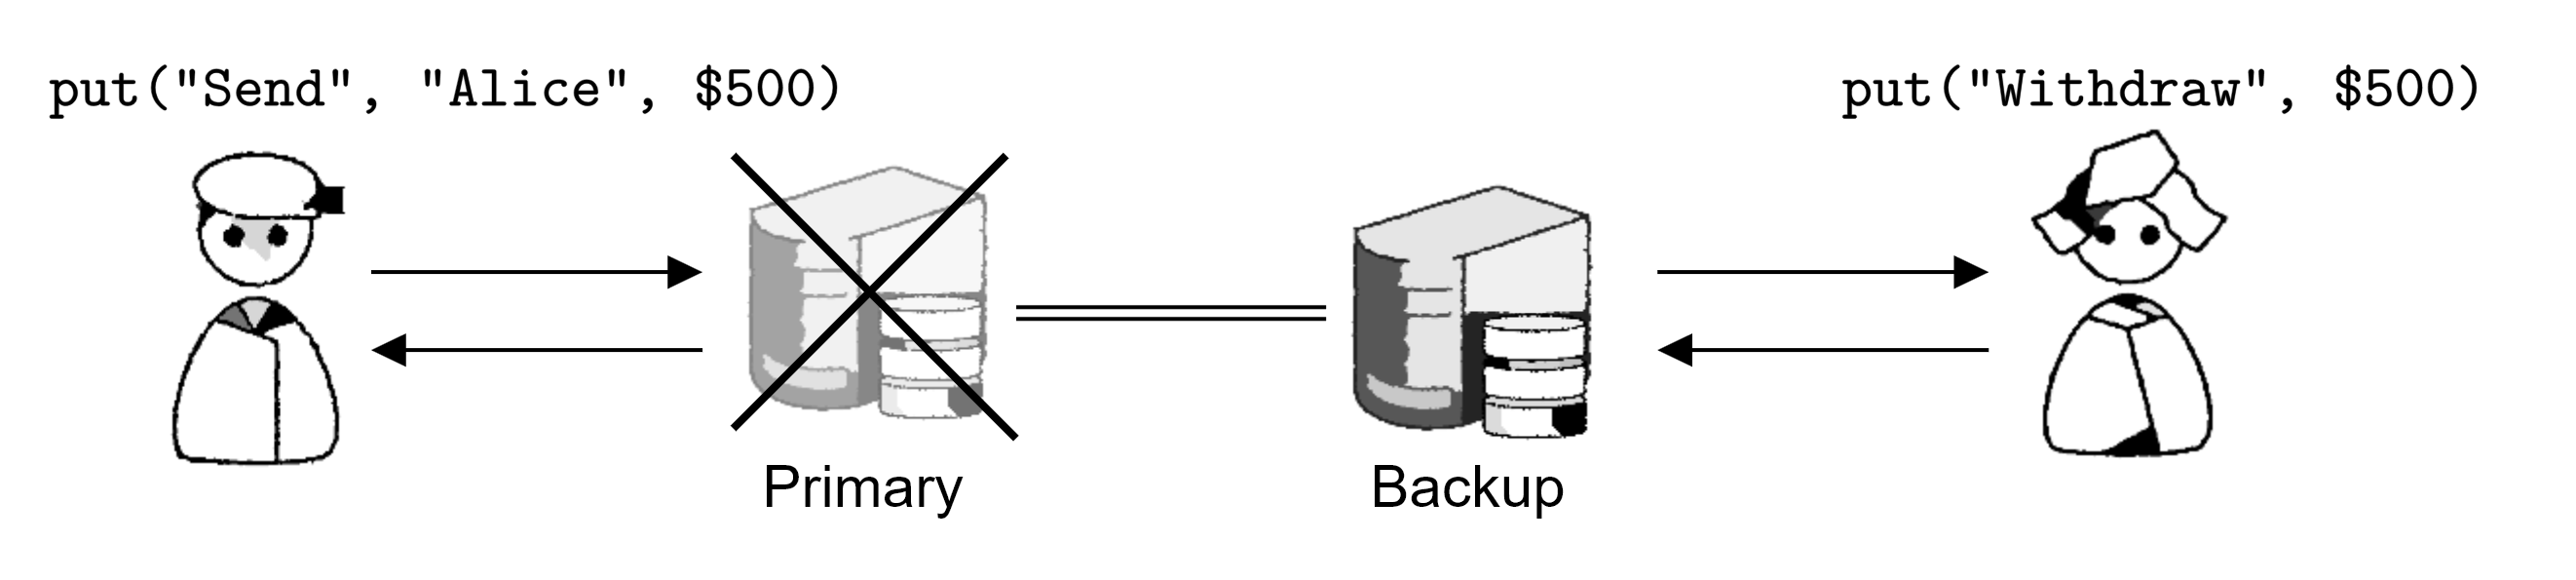
\includegraphics[width=.9\textwidth]{Sections/rep/primary.png}
    \caption{Bob's primary server failing, as Alice accesses the backup server.}
\end{figure}

\noindent
How do we ensure both parties receive consistent feedback, even when the primary server fails?
\begin{Def}[Commit Point]

    The point at which the client is committed to a transaction, goes as follows:
    \begin{enumerate}
        \item The client sends a request to the primary server and waits for an acknowledgment.
        \item The primary server forwards the request to the backup servers.
        \item The backup servers process the request and send an acknowledgment to the primary server.
        \item The primary server sends an acknowledgment to the client.
    \end{enumerate}

    \noindent
    Step 4 is considered the \textbf{commit point}.
\end{Def}

\newpage 

\noindent
The following Figure illustrates the commit point in action:
\begin{figure}[h]
    
    \hspace{1em}
    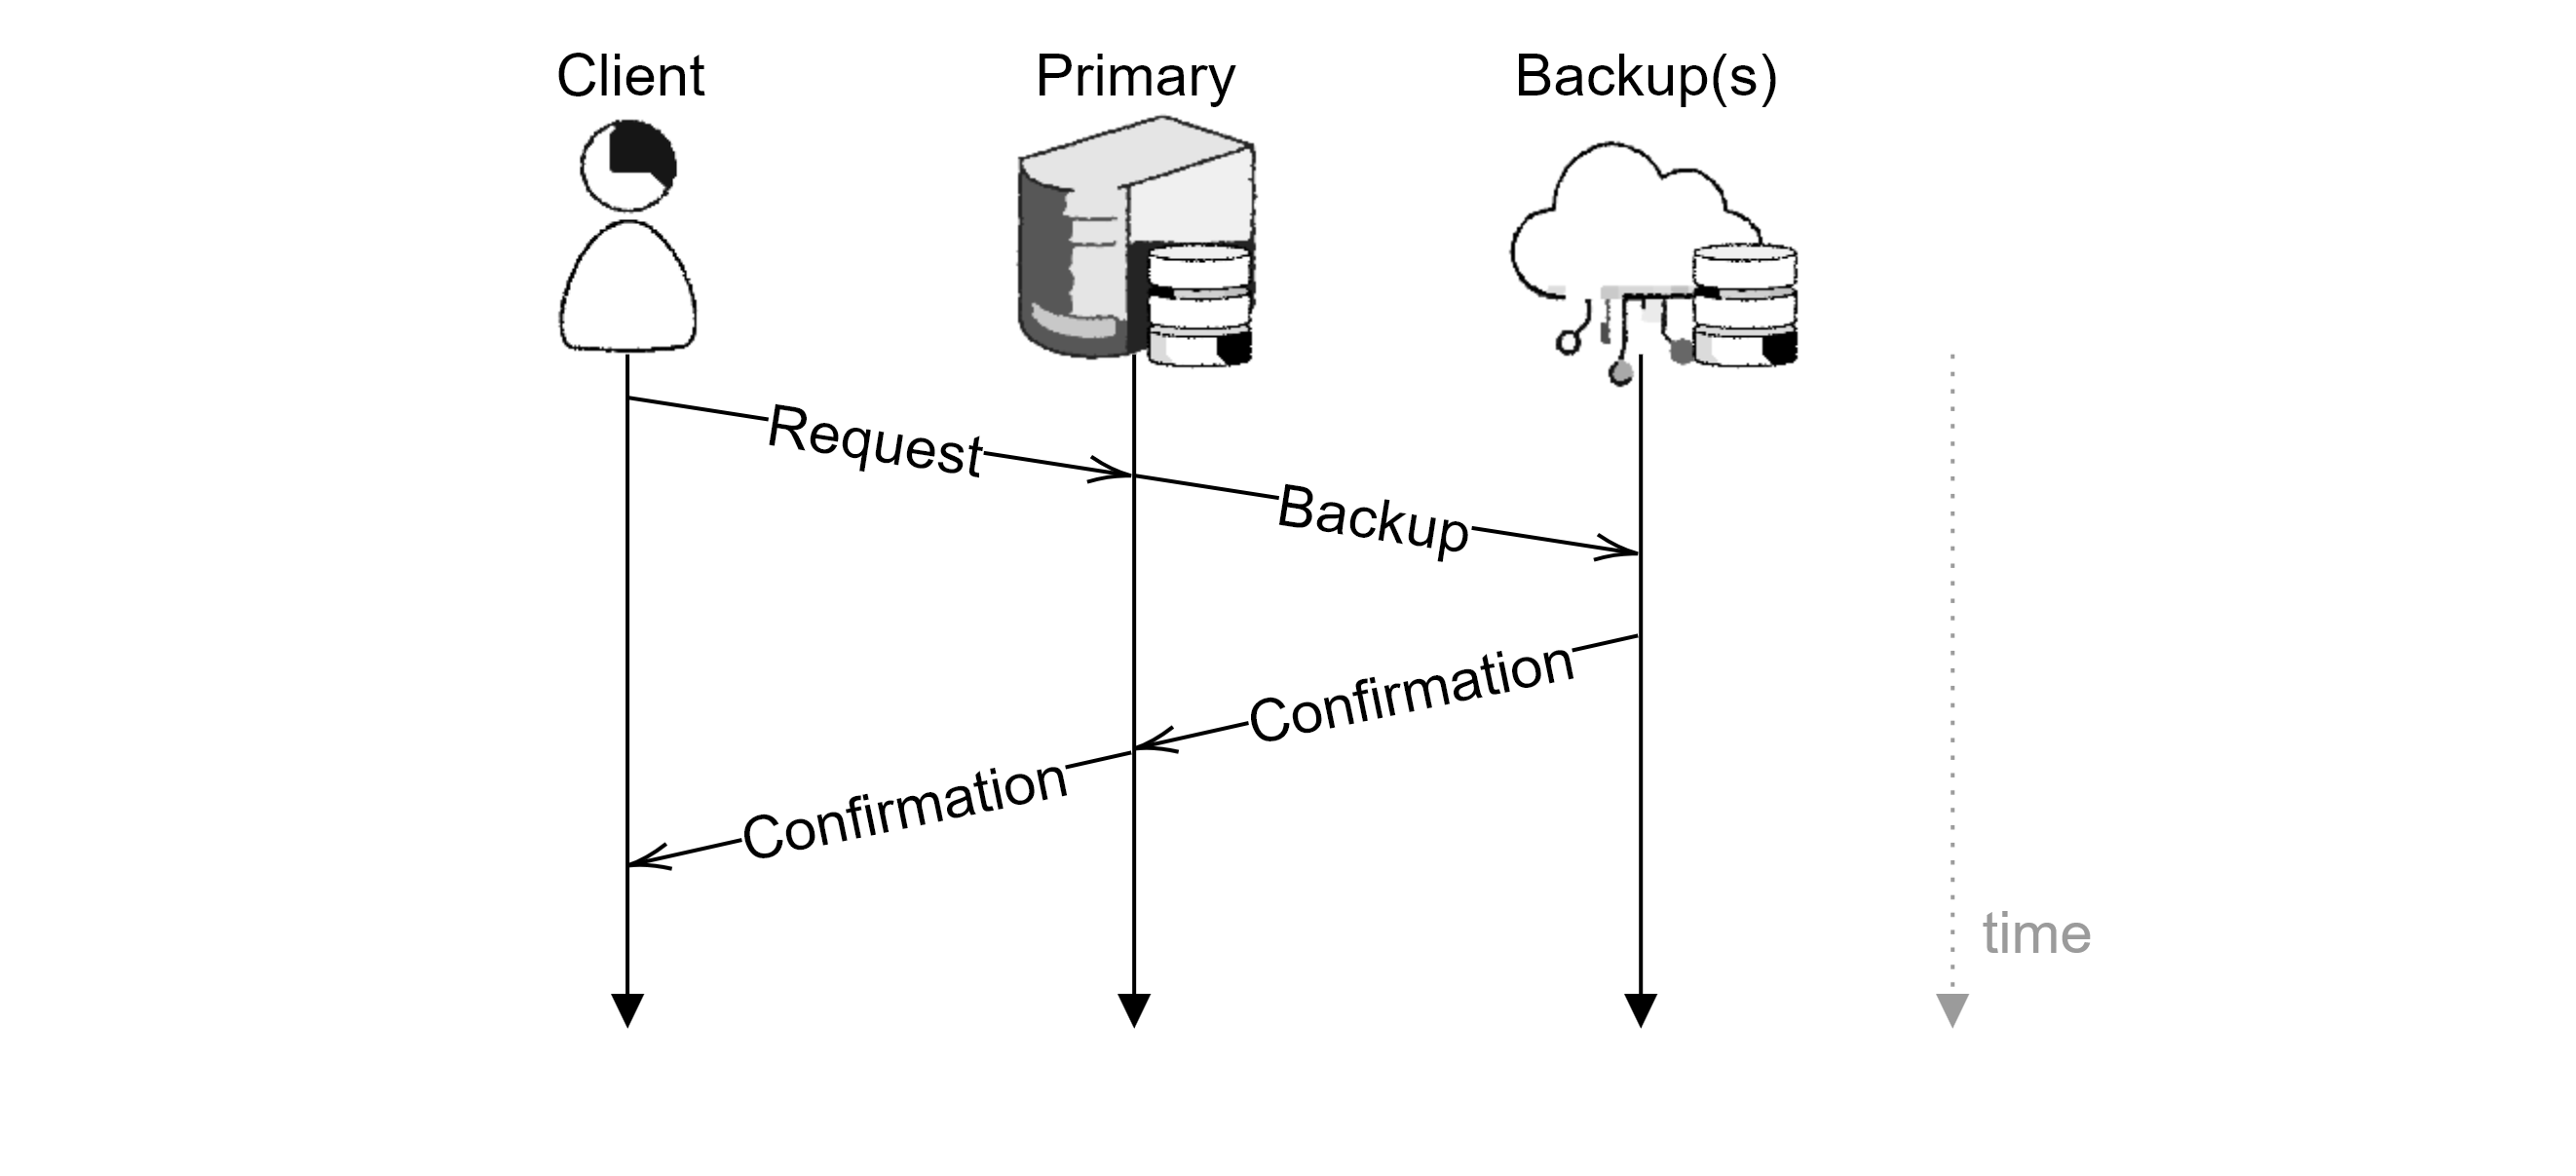
\includegraphics[width=1\textwidth]{Sections/rep/commit.png}
    \caption{Client's requests propagating through the primary and backup sever.}
\end{figure}

\noindent
We now can confirm that the client's request has been processed by the primary and backup servers, though this creates a lot of overhead as we scale the number of backups.\\

\noindent
Now that some level of consistency is ensured, we want to orchestrate designating a new primary server when the current primary server fails:

\begin{Def}[Arbitration Server and Primary Election via Test-And-Set]

    In a distributed system with a primary-backup model, maintaining a \textbf{single active primary} is crucial. When a primary server fails, a \textbf{backup must be promoted}, 
    but only if the failure is confirmed. An \textbf{Arbitration Server}, also called \textbf{Configuration Service Provider (CFG)} ensures a controlled \textbf{failover} (switching to a backup)
    process using \textbf{test-and-set}. It goes as follows:
    
    \begin{itemize}
        \item If the \textbf{primary fails} (or becomes unreachable), the CFG.
        \item The backup executes a \snippet{test\_and\_set(f,1)} operation on a shared variable \( f \).
        \begin{itemize}
            \item If \( f = 0 \), the backup sets \( f = 1 \) and becomes the new \textbf{primary}.
            \item If \( f = 1 \), another server has already taken over, preventing duplicate primaries.
        \end{itemize}
        \item Clients redirect their requests to the new primary.
    \end{itemize}
    \end{Def}
    
    \newpage
    \noindent
    To demonstrate test-and-set in action, consider the following illustration:


    \begin{figure}[h]
        
    \vspace{-1em}
        \centering
        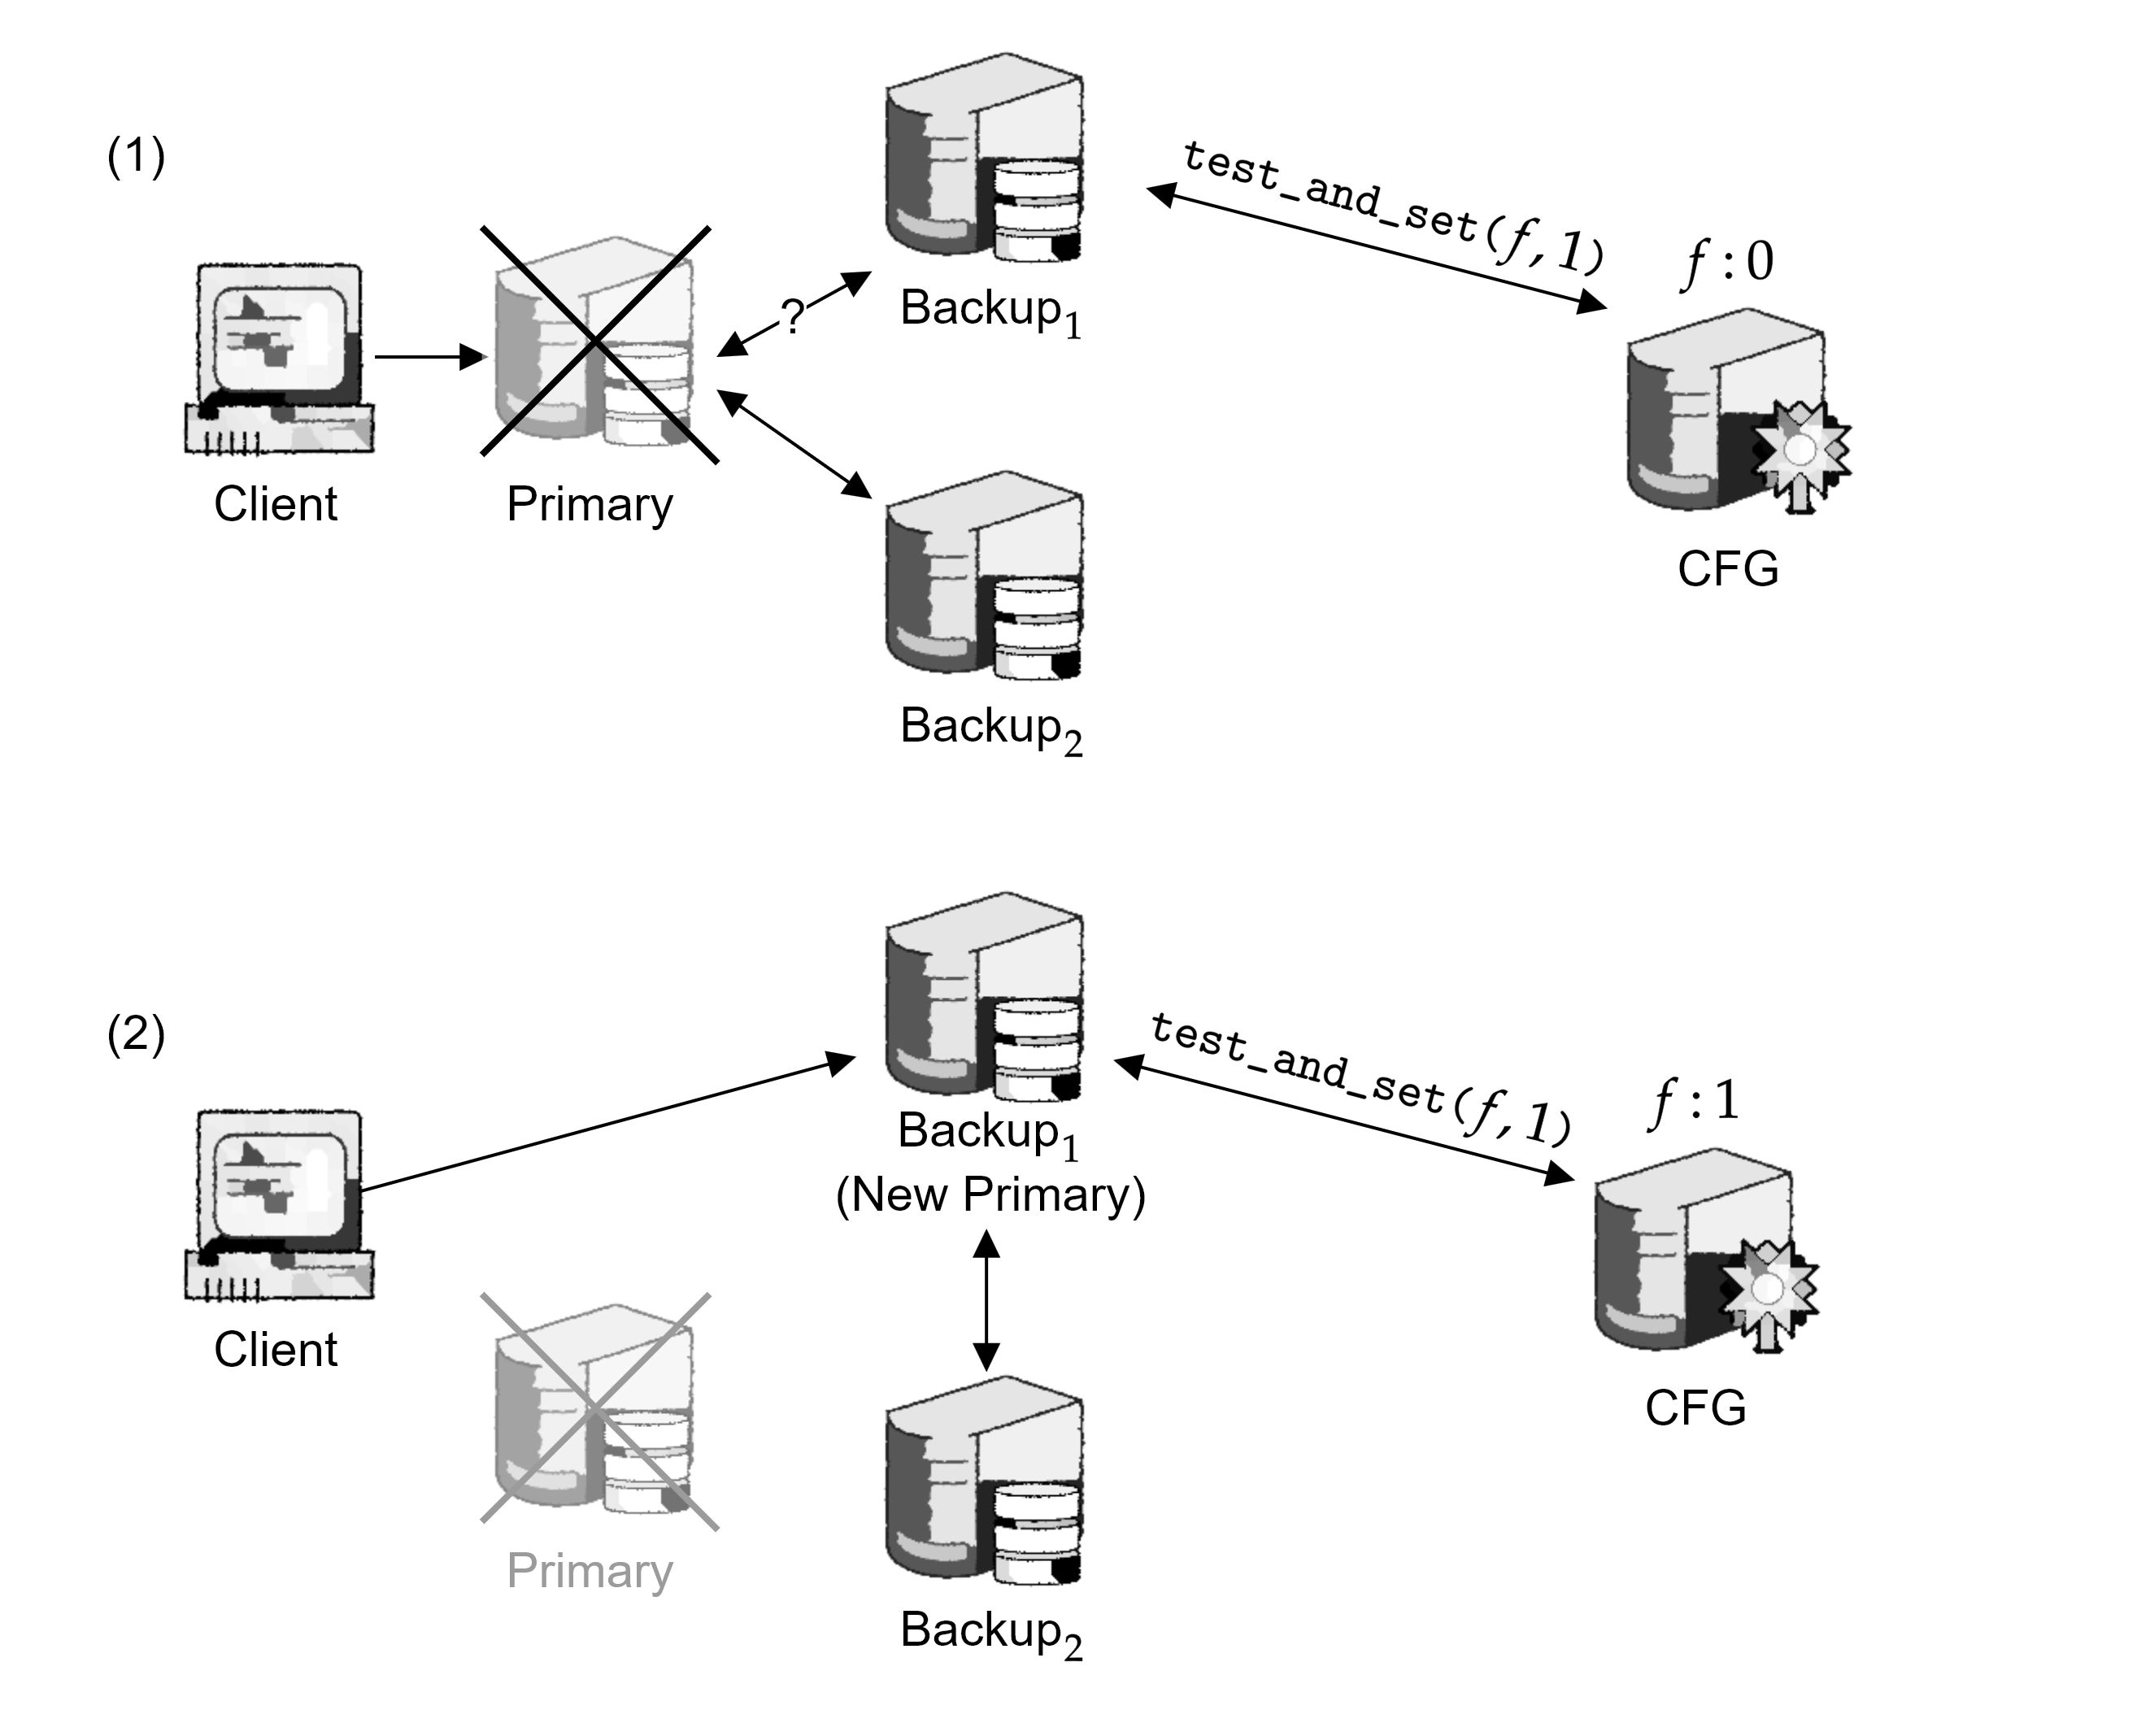
\includegraphics[width=1\textwidth]{Sections/rep/testset.png}
        \caption{Backup server 1, is unable to connect to the primary, sends promotion request to CFG. All servers are connected to the CFG with access to the shared variable \( f \). While the primary server is reachable, \( f = 0 \). When the primary fails, the backup server executes \snippet{test\_and\_set(f,1)}.}
    \end{figure}

    \noindent
    \underline{A mutex is crucial to avoid data-races} with multiple servers attempting promotion:
        \begin{lstlisting}[language=Go]
    var flag int = 0; var mu sync.Mutex;
    func (s *Server) TestAndSet(f *int, reply *int) error {
        mu.Lock()
        *reply = 0
        if flag != *f {
            flag = *f
            *reply = 1
        }
        lock.Unlock()
        return nil
    }
        \end{lstlisting}

\newpage 

\noindent
Now what if the primary server partially processed a requests before failing? Consider the following:
\begin{figure}[h]
    \centering
    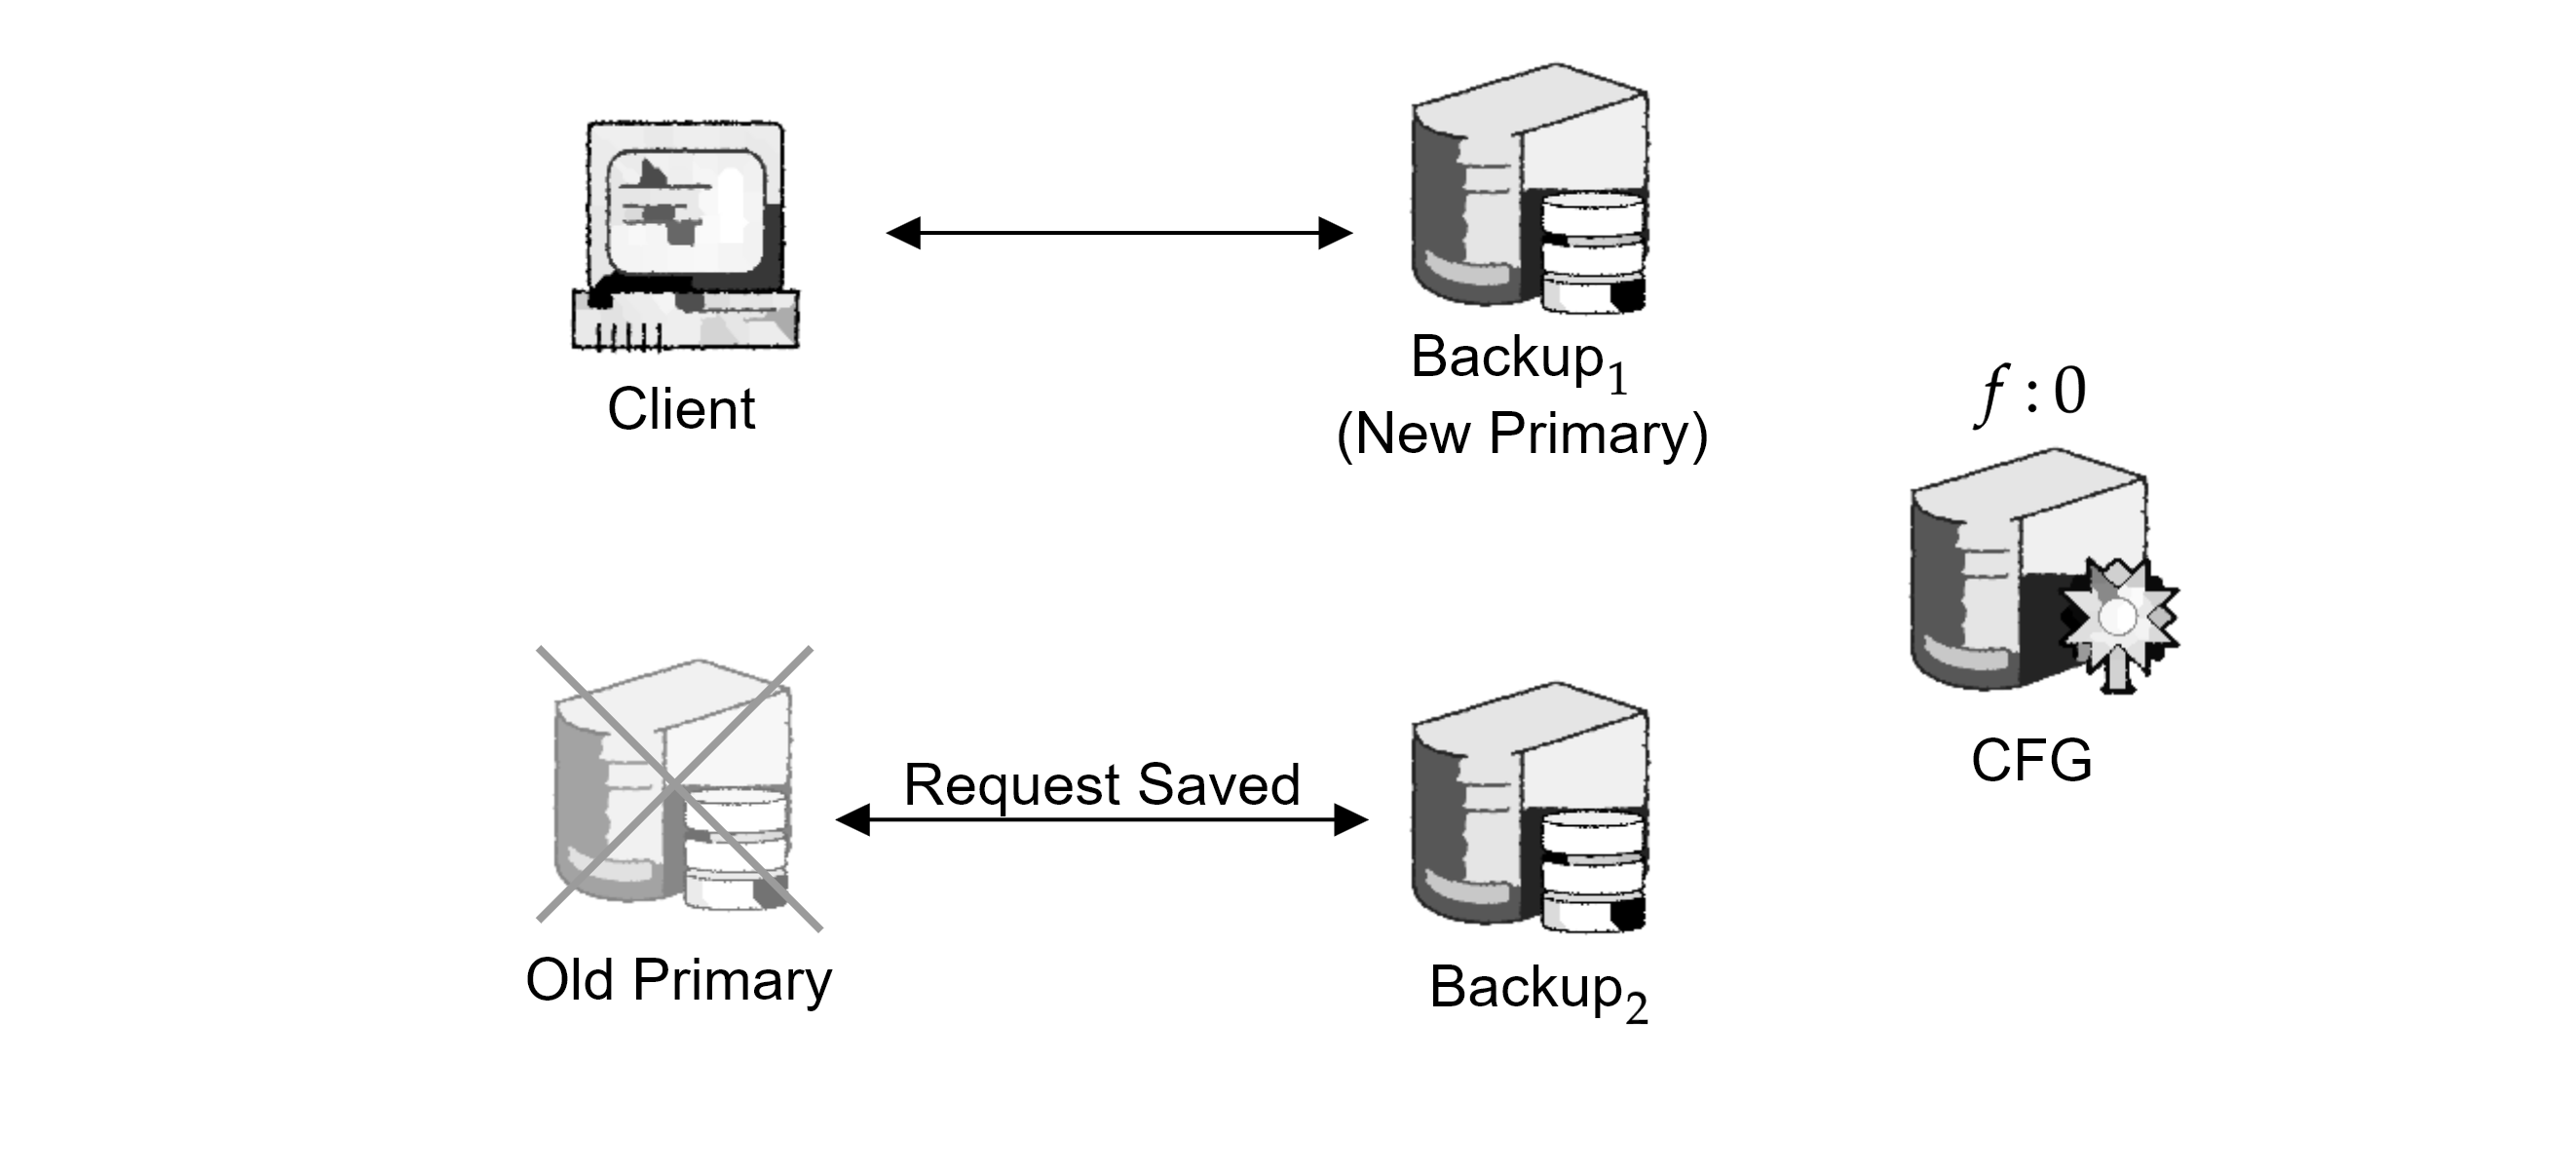
\includegraphics[width=1\textwidth]{Sections/rep/old.png}
    \caption{Primary server failing after partially processing a request.}
\end{figure}

\noindent
To combat this issue, we discuss the \textbf{Chain Replication} method:
\begin{Def}[Chain Replication]

    The \textbf{Chain Replication} architecture servers are organized in a linear sequence, forming a chain: $s_1, s_2, \ldots, s_n$, where $s_1$ is the \textbf{head} and $s_n$ is the \textbf{tail}:
    \begin{itemize}
        \item \textbf{Write Operations}: Clients send write requests to the head ($s_1$), which is forwarded to $s_2$, and so on, until the tail ($s_n$).
        \item \textbf{Read Operations}: Clients directly read from the tail ($s_n$), ensuring fully processed states; Specifically as $s_i$ states may not be fully propagated through the chain.
    \end{itemize}

    \noindent
    \textbf{Failover Handling}:
    \begin{itemize}
        \item If server $s_i$ fails, $s_{i-1}$ forwards to the successor $s_{i+1}$ instead.
        
        \item If the head ($s_1$) fails, the CFG promotes $s_2$ to be the new head.
    
        \item If the tail ($s_n$) fails, the CFG designates $s_{n-1}$ as the new tail.
    \end{itemize}

\end{Def}

\vspace{-1em}
\begin{Tip}  
    OSDI 2004 featured Robbert van Renesse and Fred B. Schneider from Cornell University, presenting Chain Replication. Van Renesse, originally from the Netherlands, and Schneider, from the U.S., have significantly influenced distributed systems research.  
    \end{Tip}
    
    
    
\noindent

Consider the comparison between \textbf{Primary-Backup} vs. \textbf{Chain Replication}:
\begin{figure}[h]
    \centering
    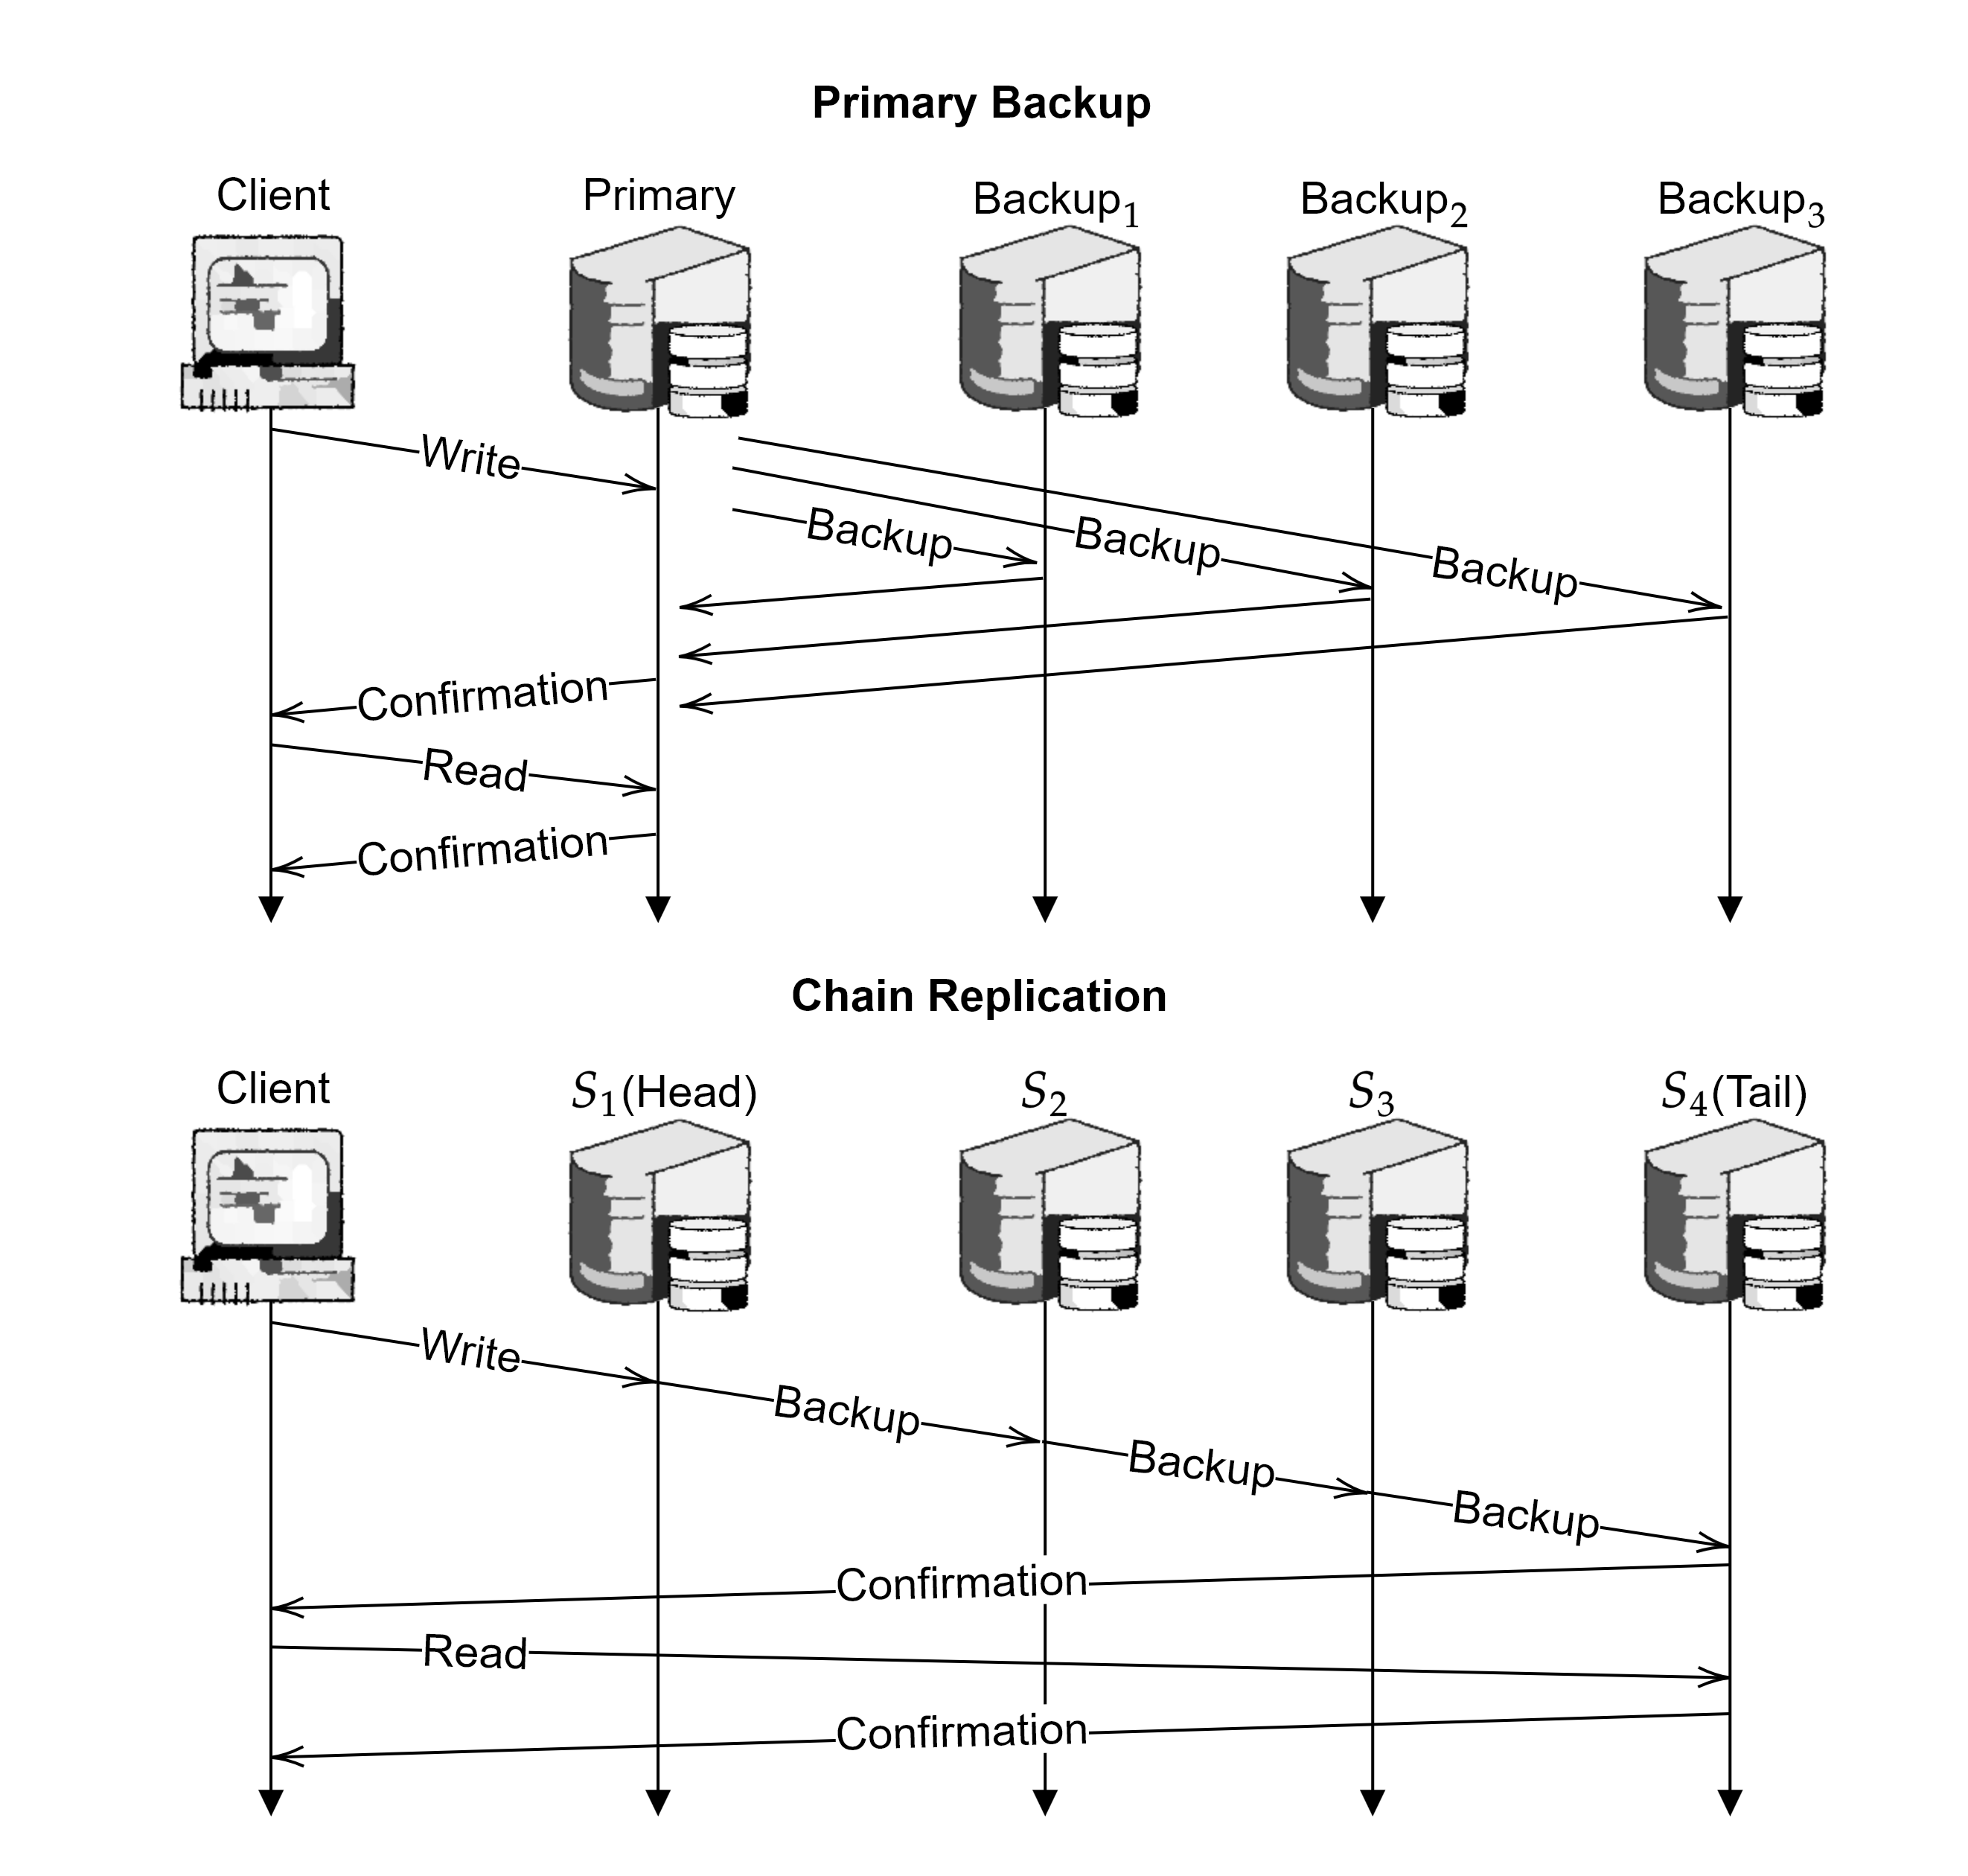
\includegraphics[width=1\textwidth]{Sections/rep/comp.png}
    \caption{Primary-Backup vs. Chain Replication}
\end{figure}

\begin{theo}[Primary-Backup vs. Chain Replication]

    In terms of \textbf{Latency}, \textbf{Primary-Backup} is faster than as the request can theoretically be processed in parallel. 
    However, \textbf{Chain Replication} is more \textbf{Fault-Tolerant} and allows for a greater degree of \textbf{Throughput}, allowing 
    requests to be processed in parallel.
\end{theo}


